\section{Ergebnisse / Evaluation}
\begin{itemize}
	\item Skalierbarkeitsgraph
	\item Wie gut ist SIMD / OpenMP / MPI / Mischformen?
	\item Frontend Overhead messen
\end{itemize}


%%%%%%%
% http://www.caps.in.tum.de/himmuc/
% Datenerhebenung (+ auf himmuc!) -> Max
% Skalierungs bzgl anzahl an nodes
% Vergleich OpenMP und mehrere MPI pro Node -> Tobi
% Overhead durch Balancer -> Florian
% Overhead durch MPI / Websocket / DrawTiles (konstant)
% Vergleich SIMD / Rohcode -> Niels

% Nutzbarkeit/ HCI -> Max
% vergleich x86 -> Max
\subsection{Performanzerhöhung alternative Parallelisierungsmechanismen}

\subsubsection{SIMD}

SIMD unterstützt in den Präzisionen 32 und 64 bit Parallelisierung von einer Rechenoperationen auf
4 beziehungsweise 2 unterschiedlichen Werten. Der Effekt beläuft sich dabei, wie in \autoref{fig:SIMD-speedup} zu sehen,
auf eine durchschnittliche Beschleunigung um den Faktor 1,9 und 1,2. %TODO hier genaue werte einsetzen

\begin{figure}
	\centering
	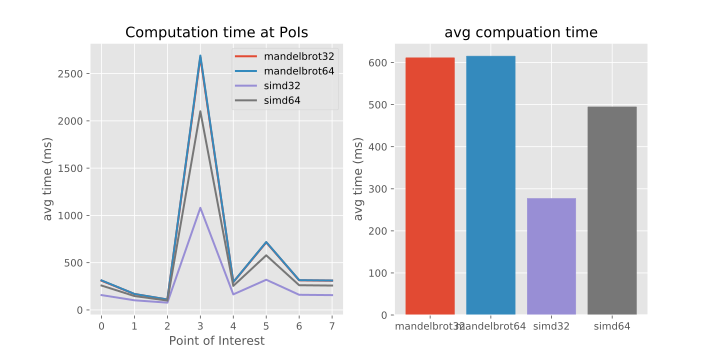
\includegraphics[width=0.9\linewidth]{img/Evaluation/impl_test}
	\caption{Vergleich der Performanzen der Implementierungen mit und ohne SIMD}
	\label{fig:SIMD-speedup}
\end{figure}

Dass die Performanzerhöhung nicht genau 4 oder 2 ist, lässt sich mit dem Erhöhten Aufwand der Verwendung
der SIMD Instruktionen erklären.
Da hierzu die Werte aus den normalen Registern in spezielle SIMD-Register und zurück
kopiert werden müssen, entsteht eine gewisse Verzögerung durch zusätzliche Schiebeoperationen.
Zudem werden für eine Menge an Punkten stets die Zahl an terationen durchgeführt,
die das Maximum aller Iterationszahlen der Punkte ist.
Dies wird dadurch bestätigt, dass die Beschleunigung am größten ist (ca. 2,5 und 1,3),
wenn alle Punkte gleich große Iterationszahlen haben.

\paragraph{Notiz, entdeckt durch das In-Betracht-Ziehen der Leerregionen}

Probleme bei der Verwendung des Rekursiven Lastbalanierers:
Da es stets im Diskreten eine Minimalgröße für die aufgeteilten Regionen gibt,
kann es sein, dass eine Region für die eine hohe Last vorhergesagt wird viele Worker reserviert -
diese jedoch nicht vollständig ausreizen kann, da die Maximalaufteilung schon erreicht wurde.
Durch die dadurch entstehenden Leerregionen von nicht verwendbaren Workern
kann eine suboptimale Aufteilung enstehen, schlechter noch als die des naiven rekursiven Balancierers.

Dies kann abgeschwächt werden, indem eine Region stets nur soviel Workerressourcen erhält,
wie sie maximal auslasten könnte (Fläche/Fläche minimaler Aufteilung)
